% Appendix1 file from standard thesis template

\appendixtitle 
\appendix

%% Use the following two lines for single appendix
%\unappendixtitle
%\singleappendixtitle

\chapter{}

\begin{figure}\
  \begin{subfigure}[b]{0.49\textwidth}
    \centering
    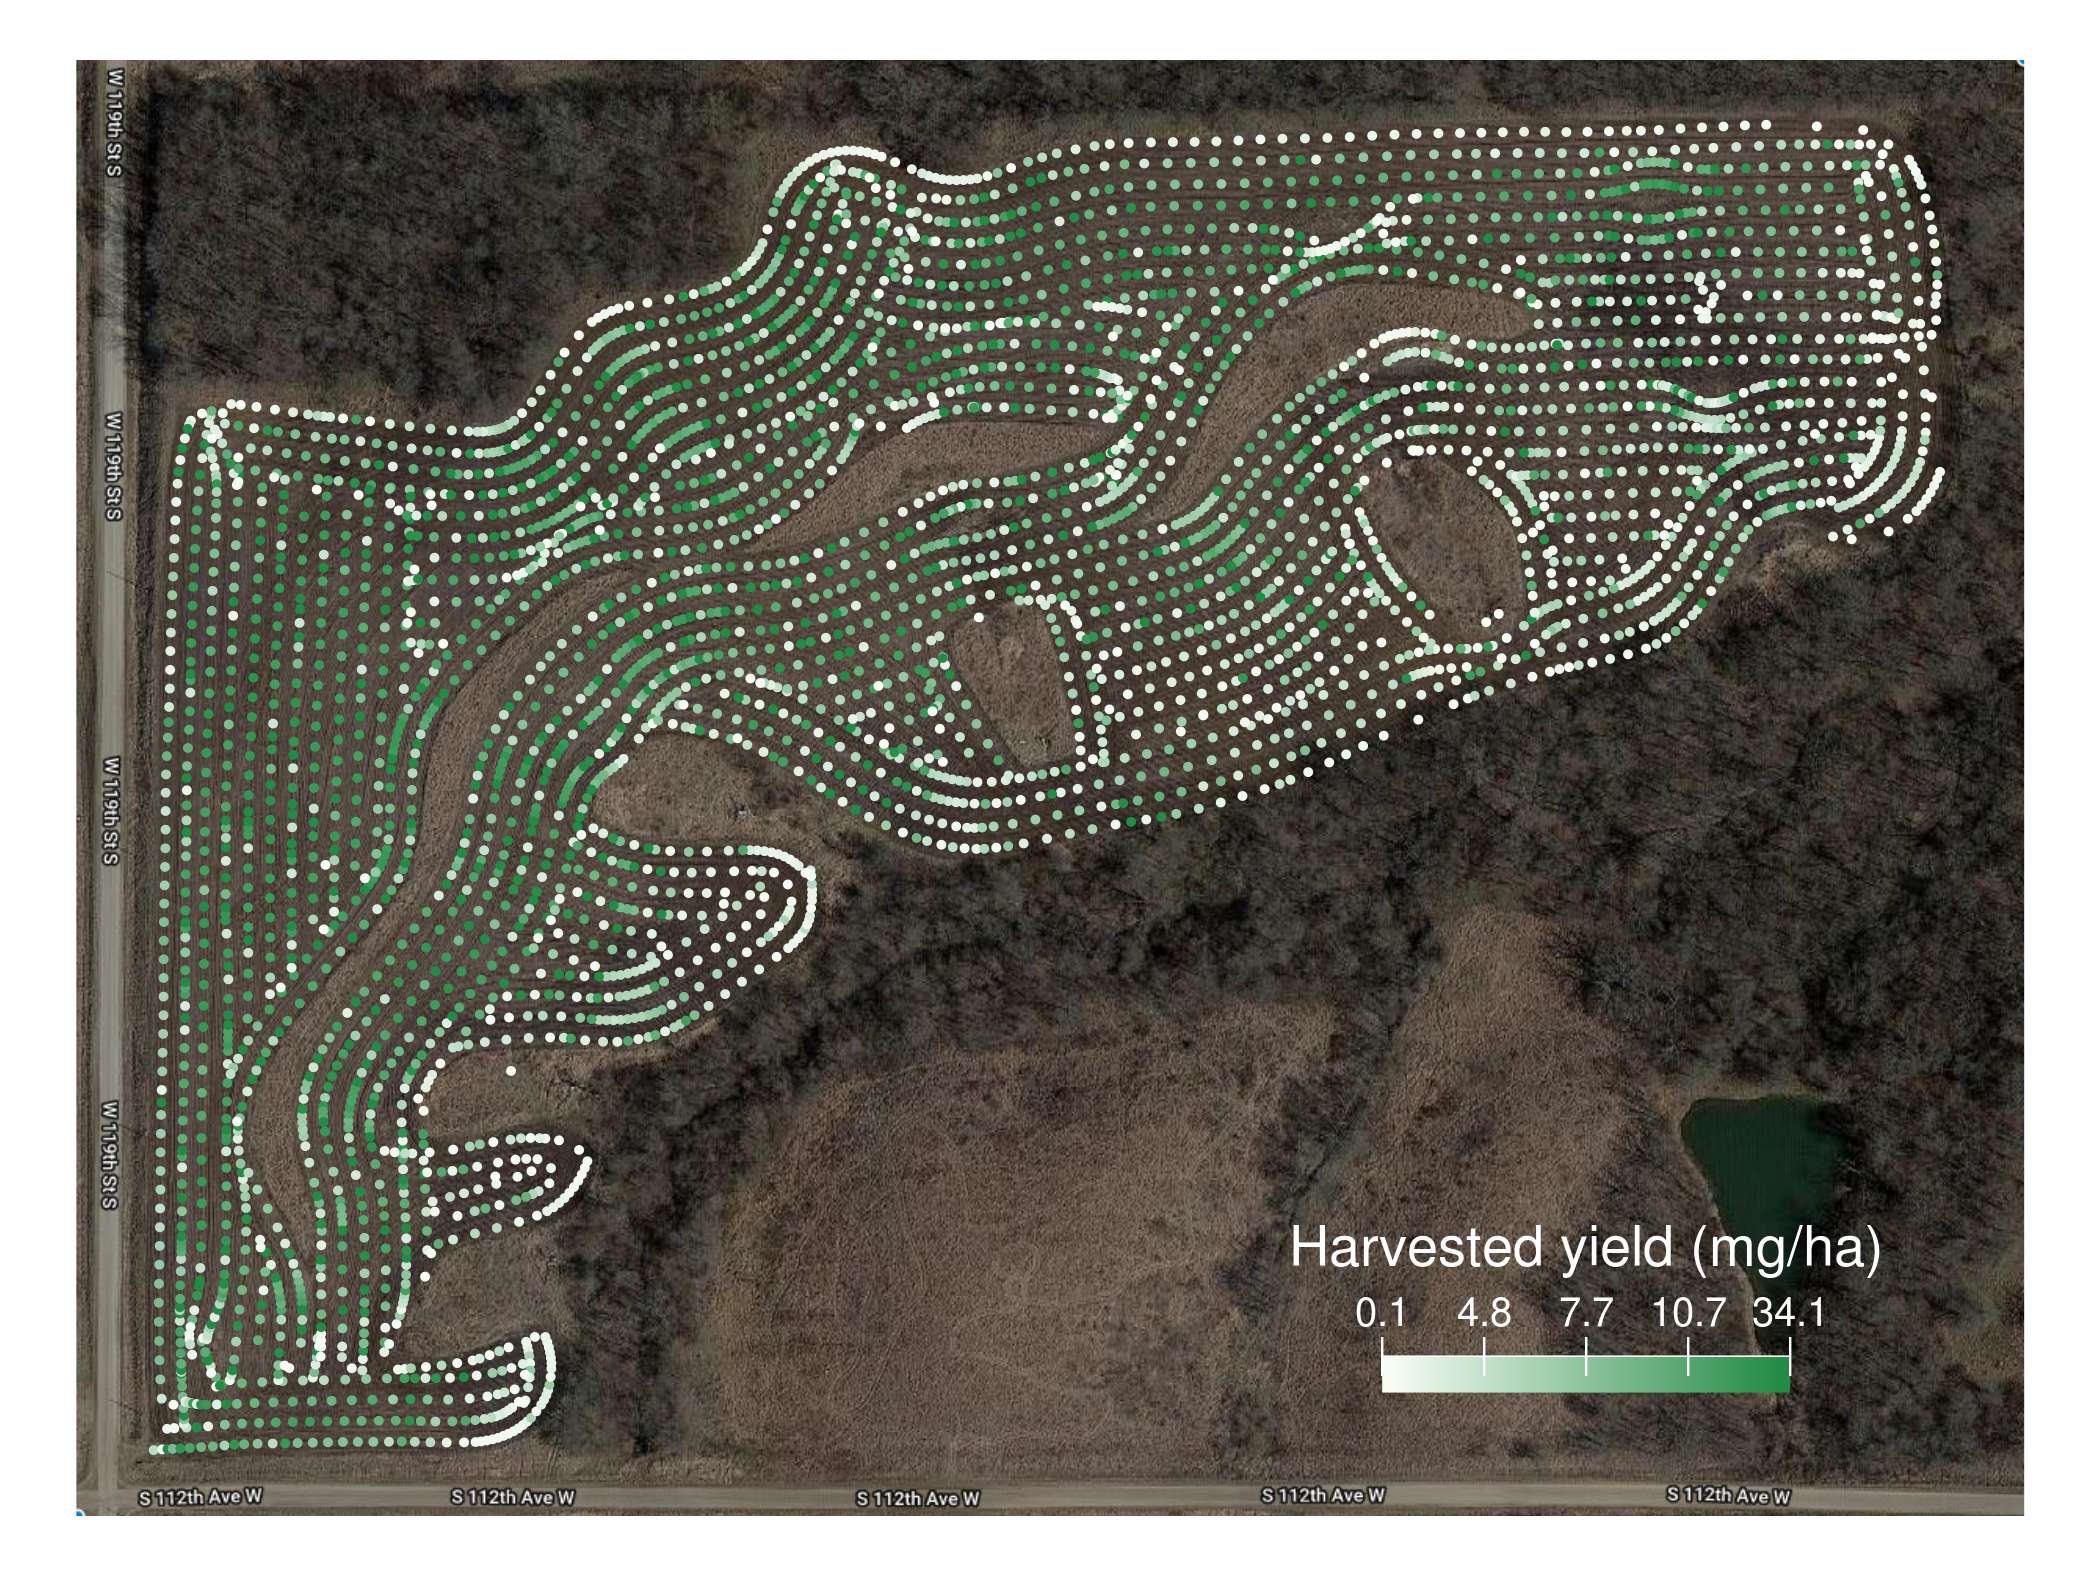
\includegraphics[width=1\textwidth]{appendix/basswood_2012_res5_1_points_vehicle}
    \caption{Observations as point on a 2D-space}
   \end{subfigure}
  \begin{subfigure}[b]{0.49\textwidth}
    \centering
    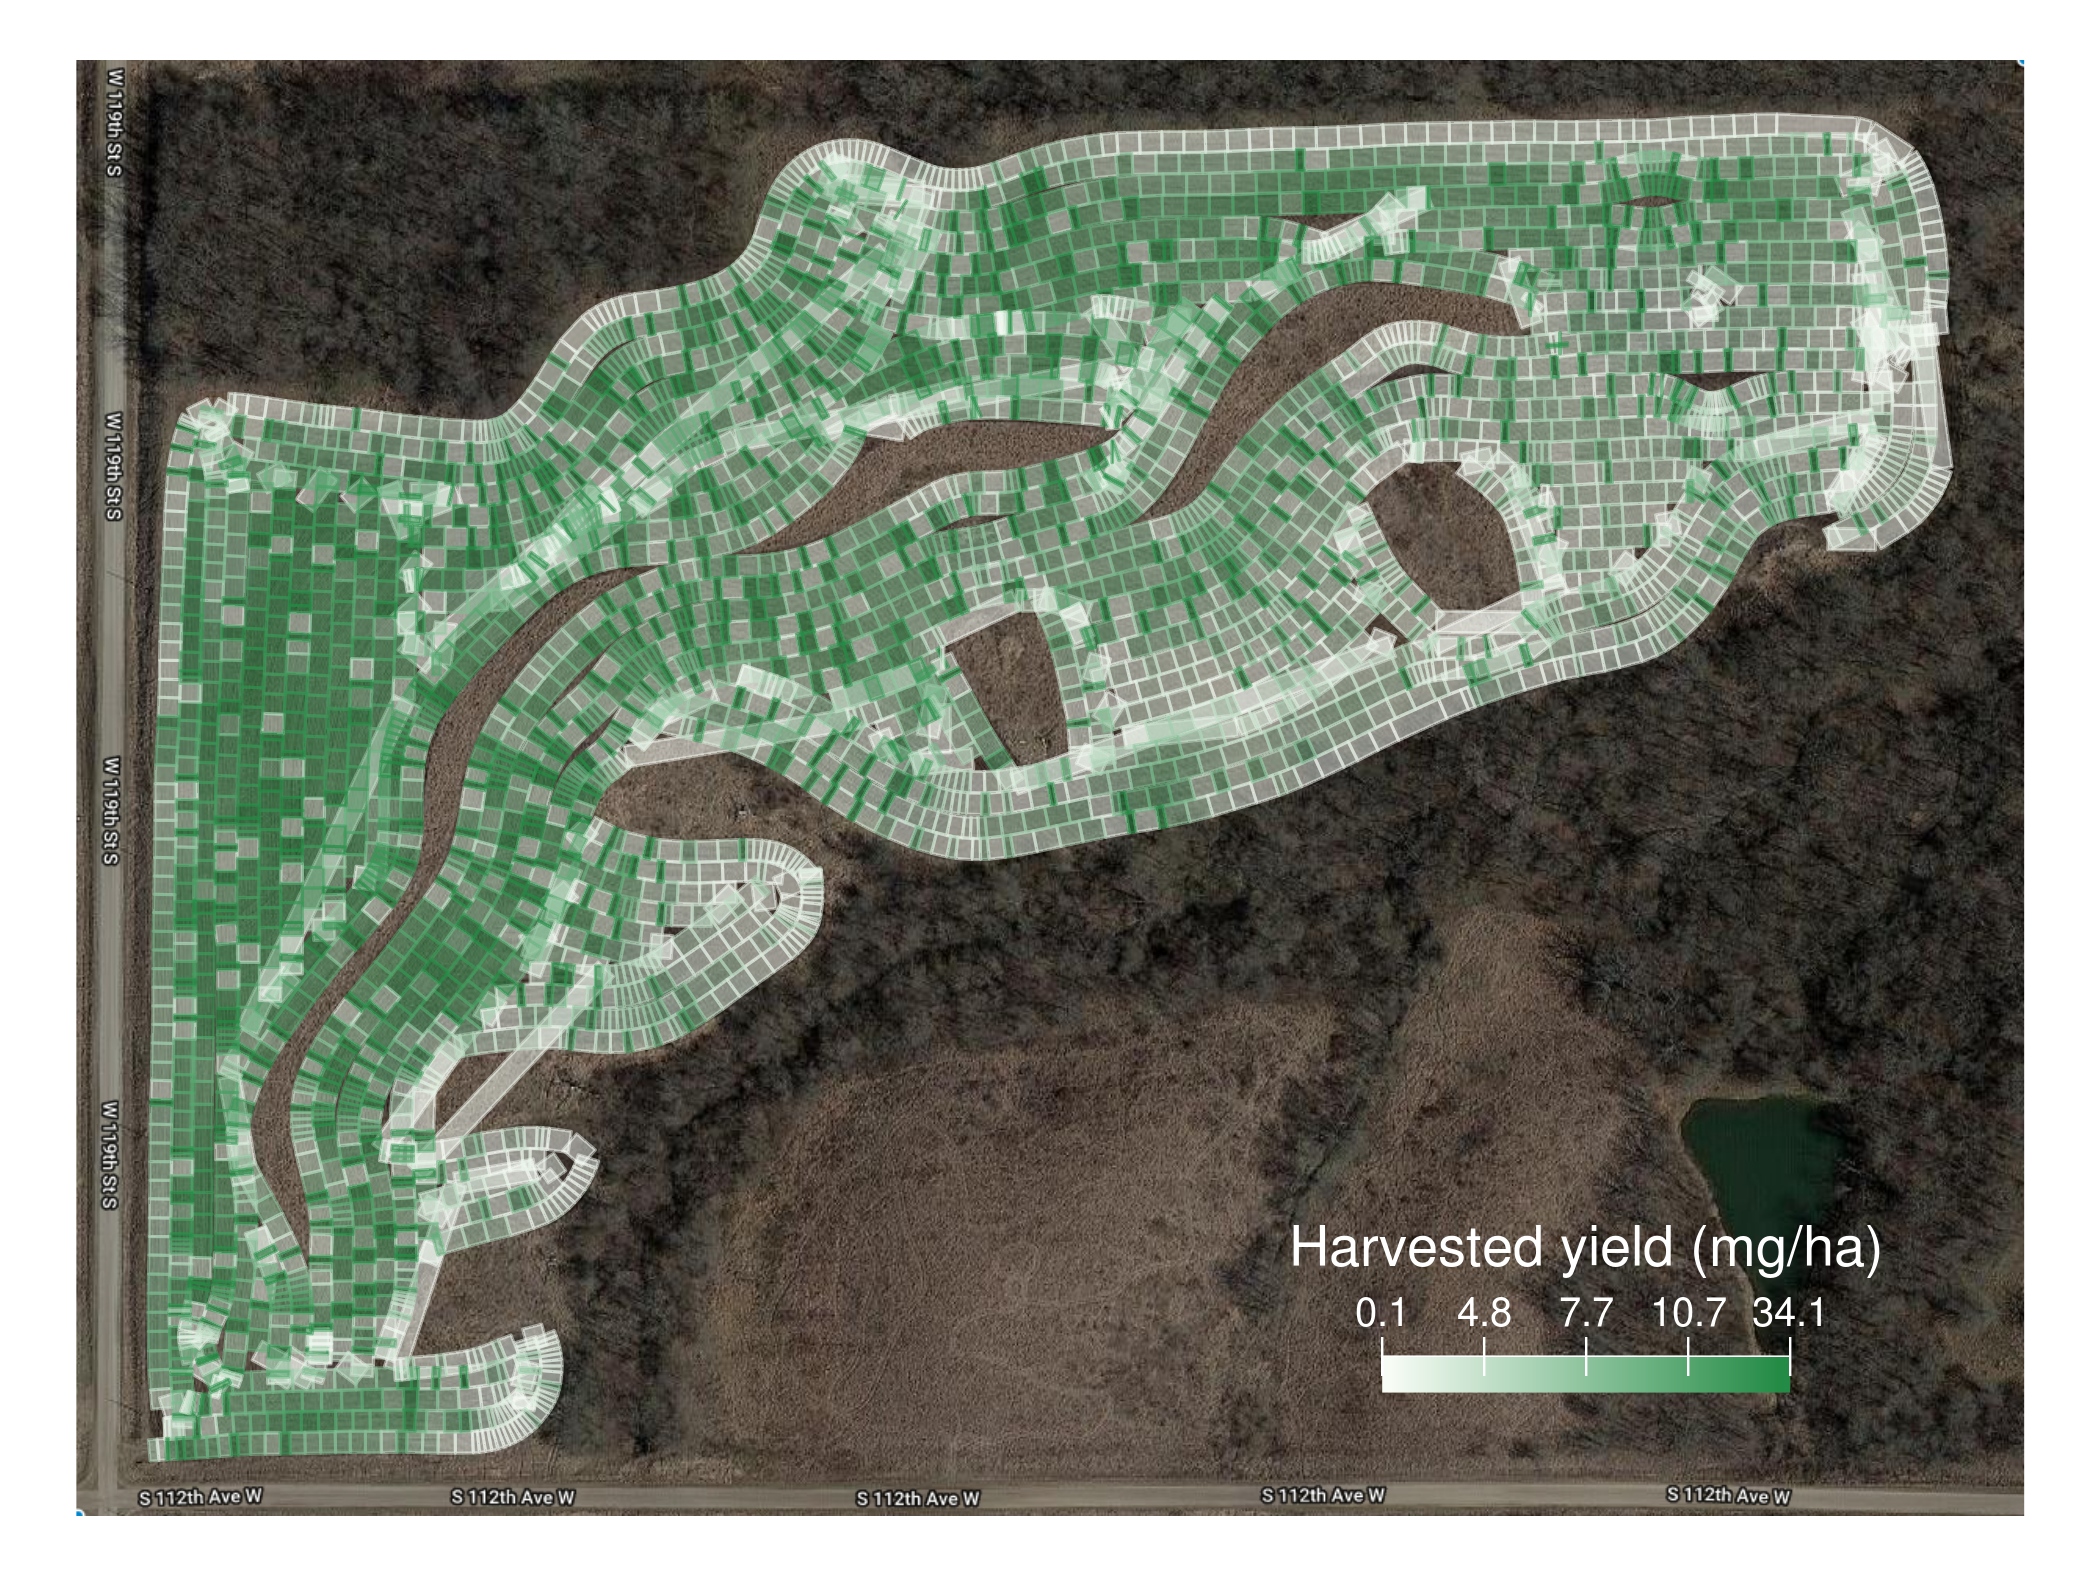
\includegraphics[width=1\textwidth]{appendix/basswood_2012_res5_1_polygons_vehicle}
    \caption{Rectangle creation step output}
  \end{subfigure}
  \begin{subfigure}[b]{0.49\textwidth}
    \centering
    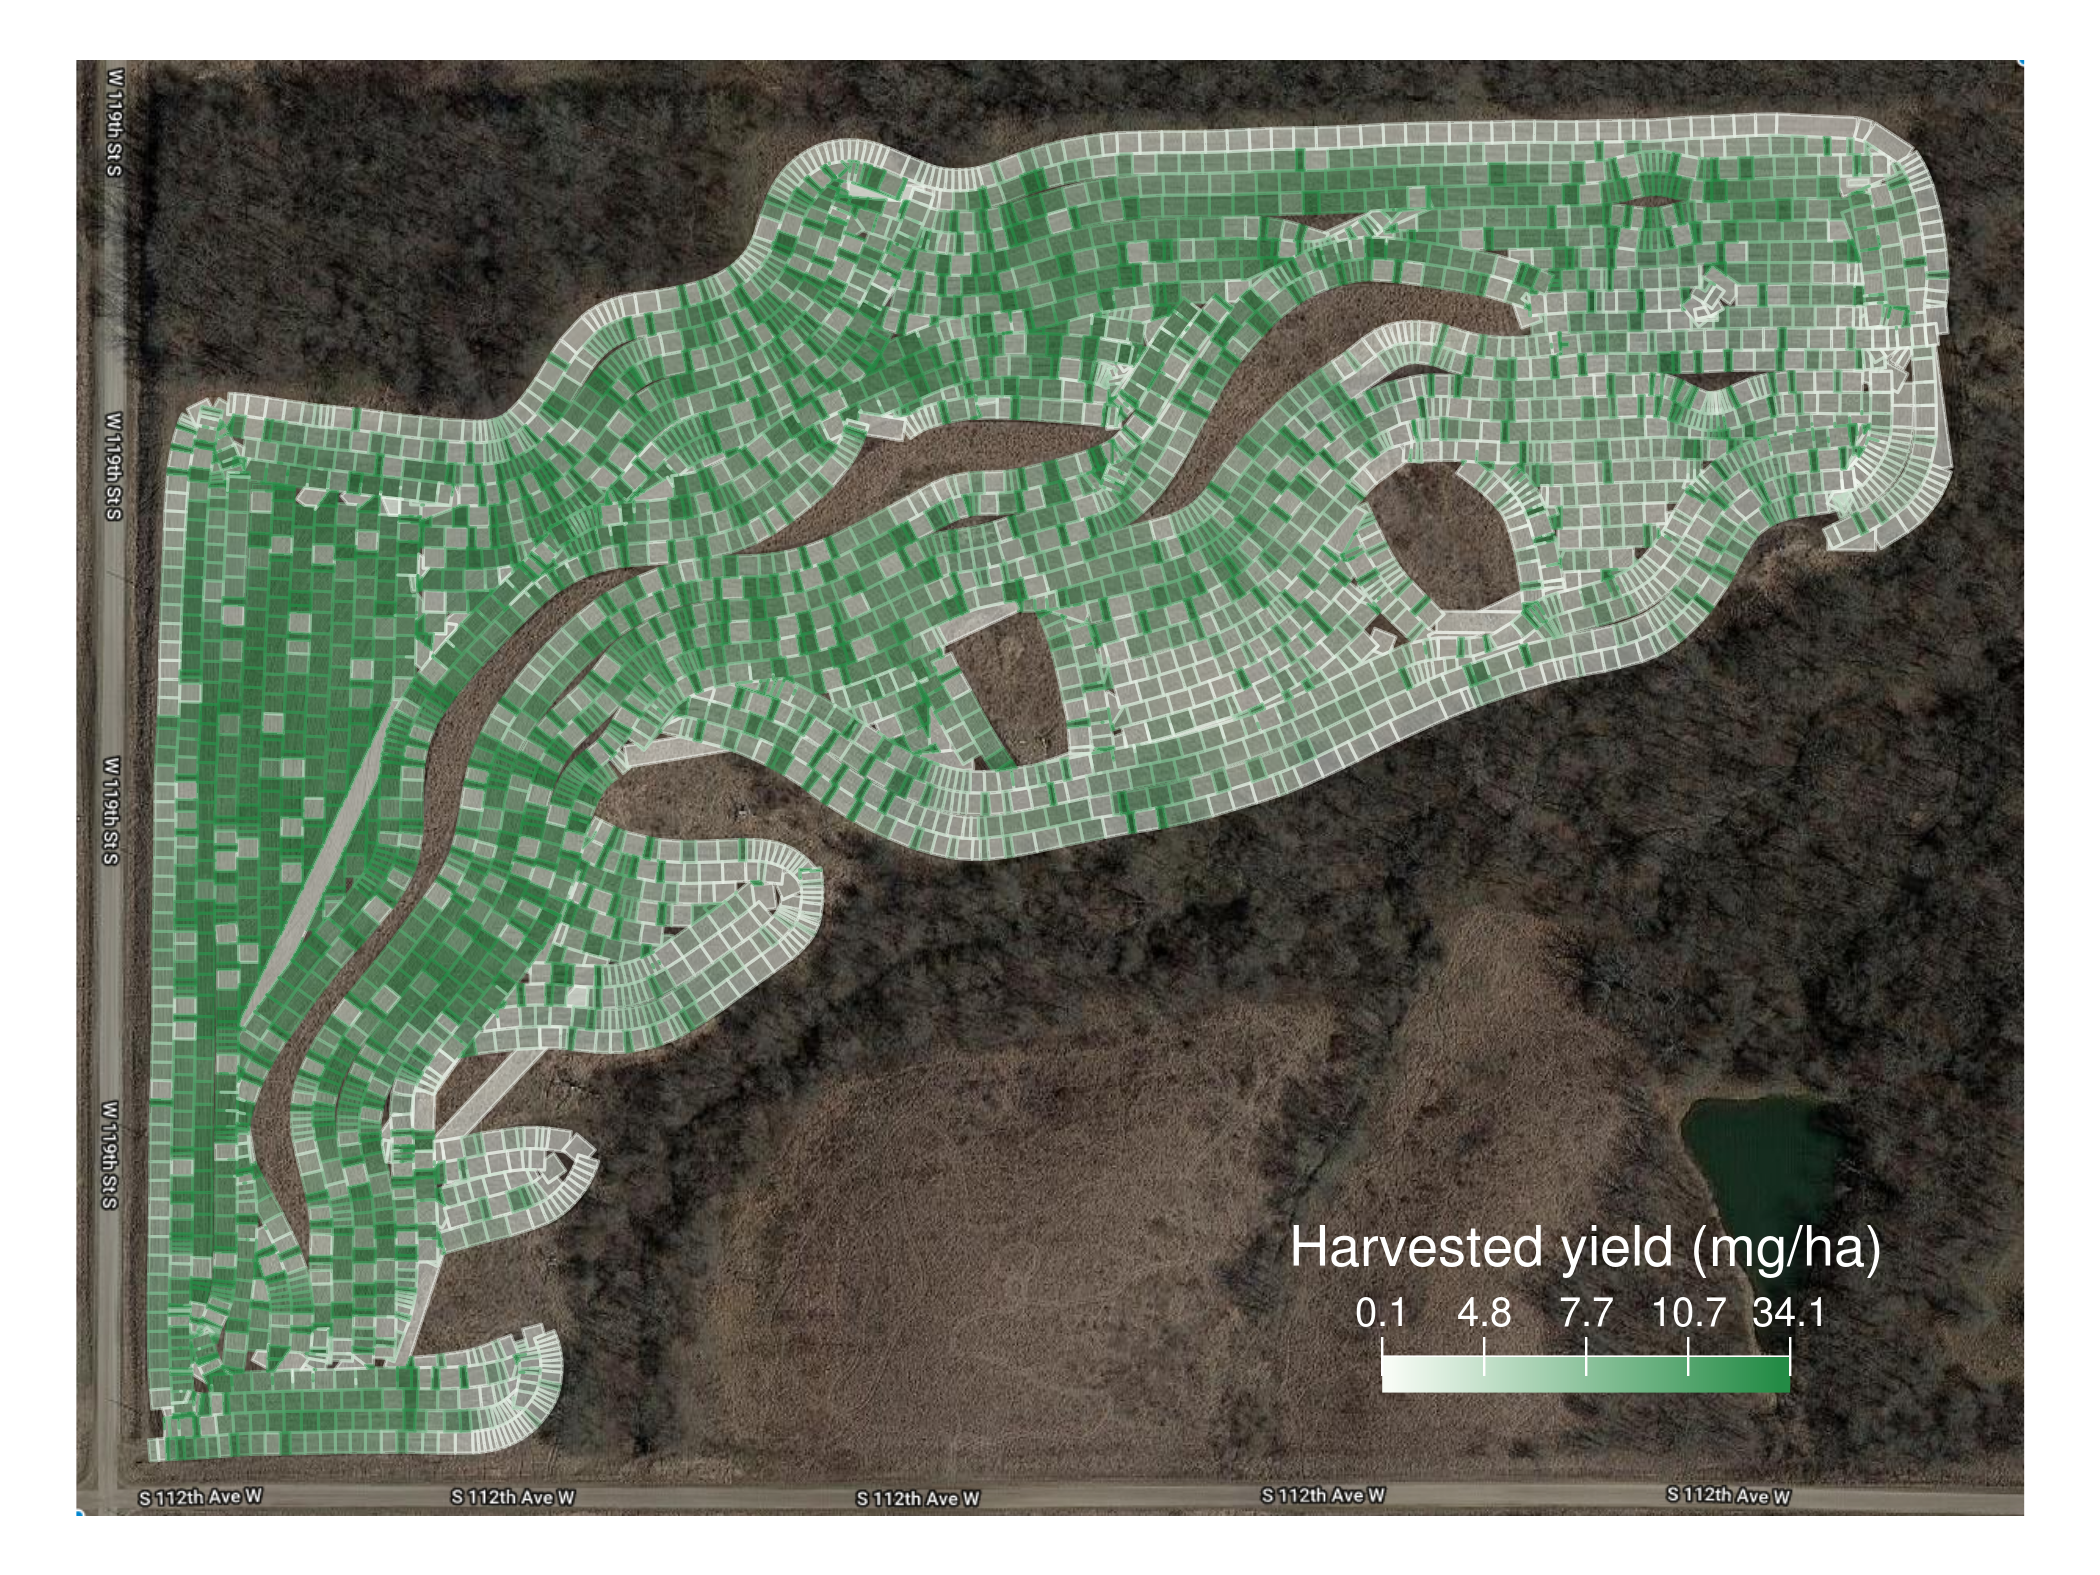
\includegraphics[width=1\textwidth]{appendix/basswood_2012_res5_1_reshaped}
    \caption{Tessellation step output}
  \end{subfigure}
  \begin{subfigure}[b]{0.49\textwidth}
    \centering
    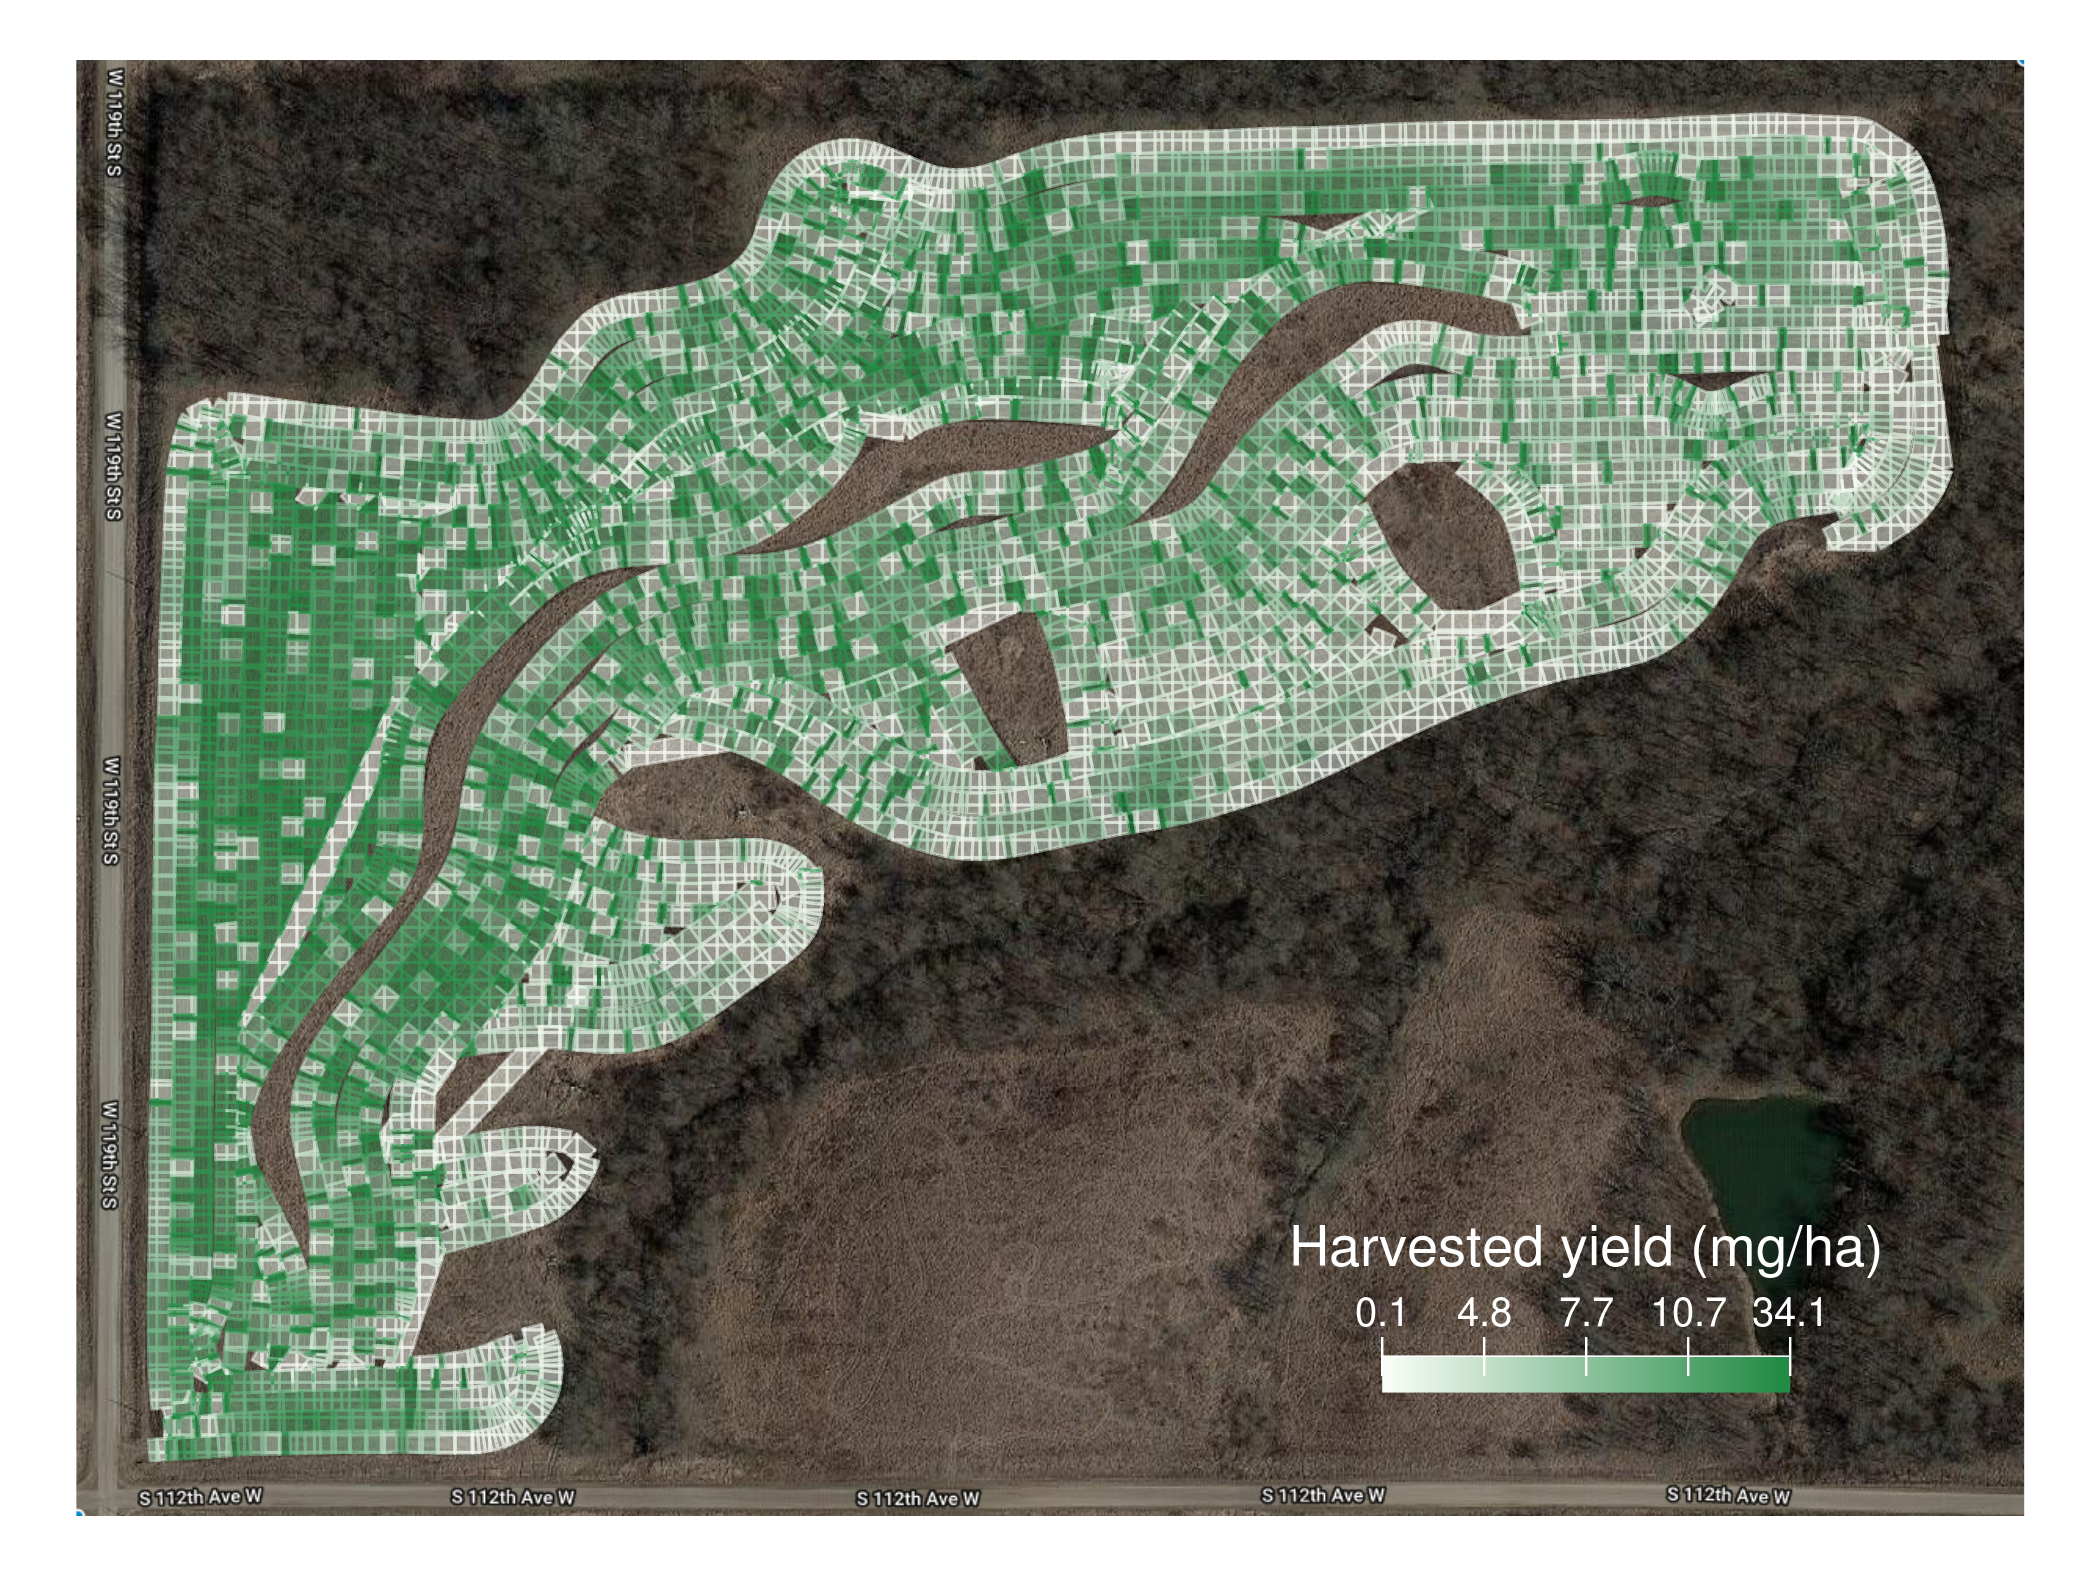
\includegraphics[width=1\textwidth]{appendix/basswood_2012_res5_1_chopped}
    \caption{Tessellated plane partition}
   \end{subfigure}
  \begin{subfigure}[b]{0.49\textwidth}
    \centering
    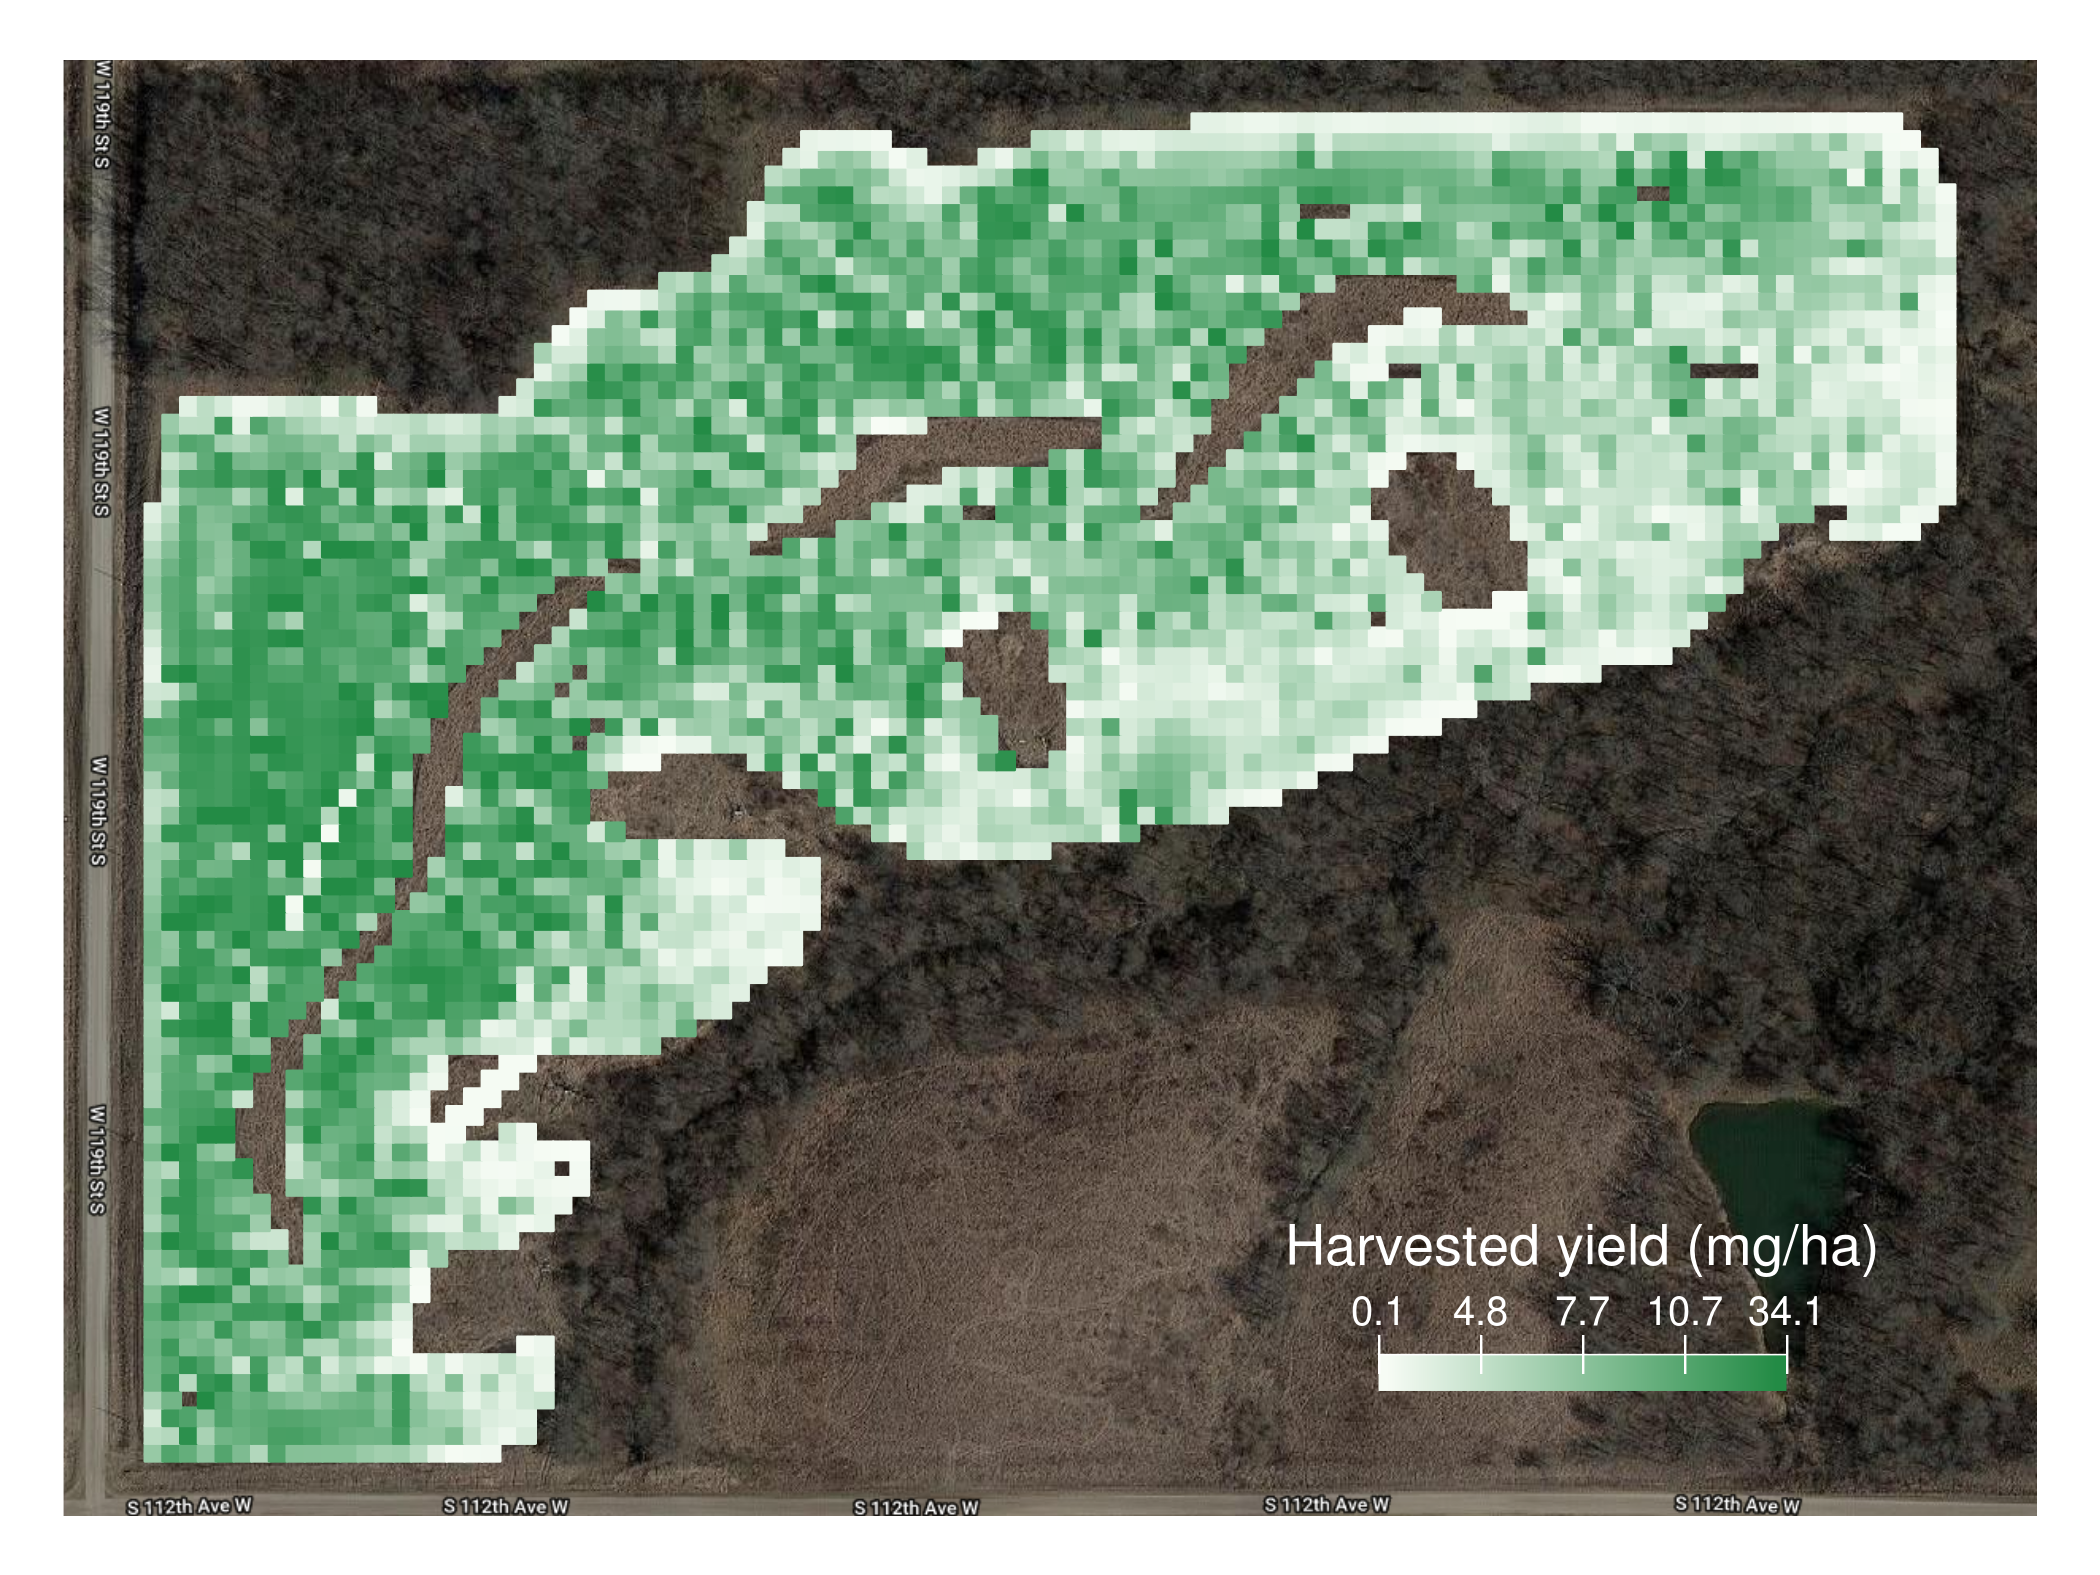
\includegraphics[width=1\textwidth]{appendix/basswood_2012_res5_1_aggregated}
    \caption{Apportioning step output}
  \end{subfigure}
  \begin{subfigure}[b]{0.49\textwidth}
    \centering
    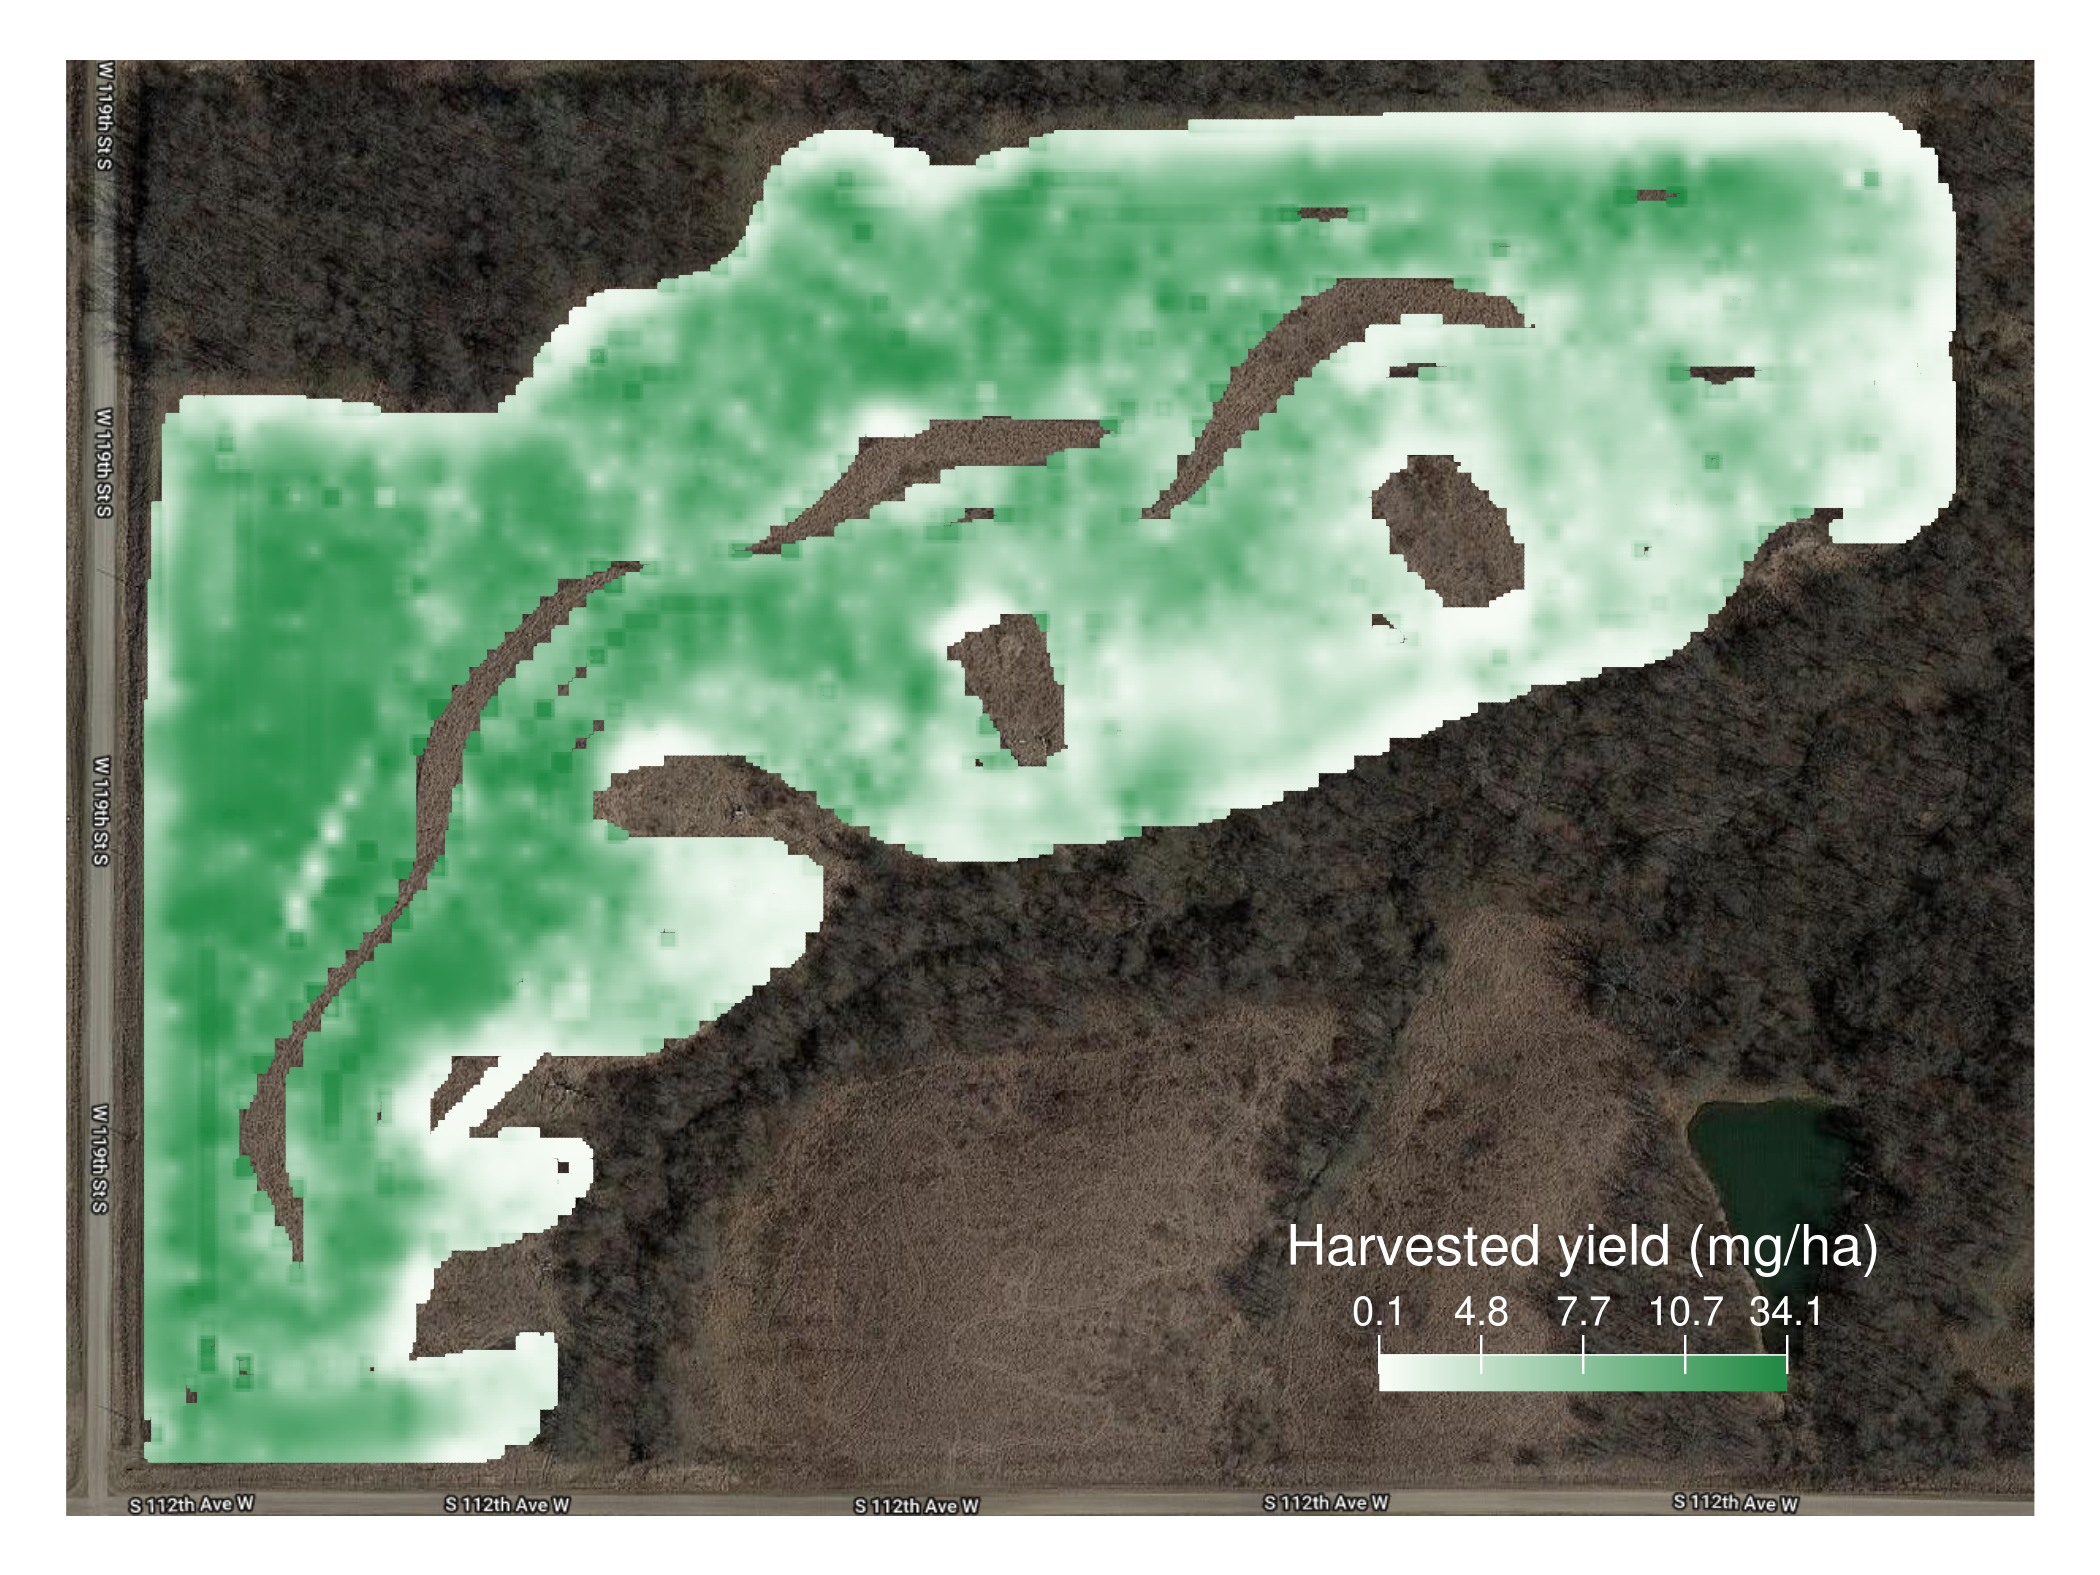
\includegraphics[width=1\textwidth]{appendix/basswood_2012_res5_1_smoothed}
    \caption{Smoothing step output}
  \end{subfigure}
  \caption[Step-by-step visualization of the algorithm for one
  field]{Step-by-step progression of Basswood (2012).}
  \label{fig:basswood2012-all-steps}
\end{figure}

%%% Local Variables:
%%% mode: latex
%%% TeX-master: "../thesis"
%%% End:
